\begin{figure}[H]
    \centering


\resizebox{\linewidth*3/4}{!}{
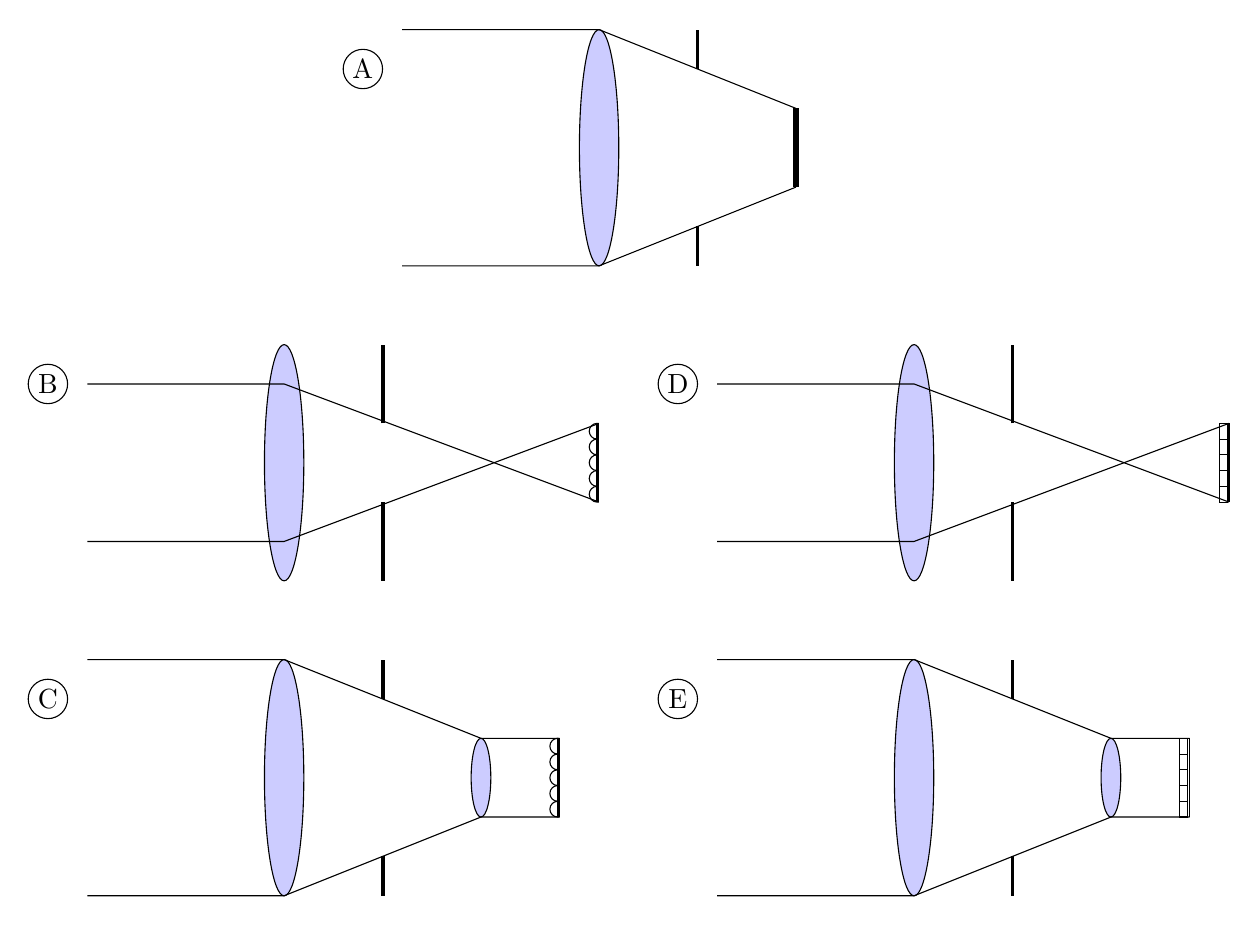
\begin{tikzpicture}[scale=.5]

%%%%%% low F-number, no microlens

%lens
\draw [fill=blue!20] (7,4) ellipse (0.5 and 3);

%diafragma
\draw [line width=.5mm] (9.5,6) -- (9.5,7);
\draw [line width=.5mm] (9.5,1) -- (9.5,2);

%sensitive area
\draw [line width=.7mm] (12,3) -- (12,5);

%light beams
\draw (2,7) to (7,7) to (12,5);
\draw (2,1) to (7,1) to (12,3);

%%%%%%Microlens + high F-number

%lens
\draw [fill=blue!20] (-1,-4) ellipse (0.5 and 3);

%diafragma
\draw [line width=.5mm] (1.5,-3) -- (1.5,-1);
\draw [line width=.5mm] (1.5,-7) -- (1.5,-5);

%sensitive area
\draw [line width=.7mm] (7,-5) -- (7,-3);

%light beams
\draw (-6,-2) to (-1,-2) to (7,-5);
\draw (-6,-6) to (-1,-6) to (7,-3) node (v1) {};


%Microlenses
\draw  (6.95,-3.2) ellipse (.2 and .2);
\draw  (6.95,-3.6) ellipse (.2 and .2);
\draw  (6.95,-4.0) ellipse (.2 and .2);
\draw  (6.95,-4.4) ellipse (.2 and .2);
\draw  (6.95,-4.8) ellipse (.2 and .2);
\fill  (7,-2.8) rectangle (7.4,-5.2) [fill=white];

%%%%%%Microlens + extra lens

%lens
\draw [fill=blue!20] (-1,-12) ellipse (0.5 and 3);

%second lens
\draw [fill=blue!20] (4,-12) ellipse (0.25 and 1);

%diafragma
\draw [line width=.5mm] (1.5,-10) -- (1.5,-9);
\draw [line width=.5mm] (1.5,-15) -- (1.5,-14);

%sensitive area
\draw [line width=.75mm] (6,-13) -- (6,-11);

%light beams
\draw (-6,-9) to (-1,-9) to (4,-11) to (6,-11);
\draw (-6,-15) to (-1,-15) to (4,-13) to (6,-13);


%Microlenses
\draw  (5.95,-11.2) ellipse (.2 and .2);
\draw  (5.95,-11.6) ellipse (.2 and .2);
\draw  (5.95,-12) ellipse (.2 and .2);
\draw  (5.95,-12.4) ellipse (.2 and .2);
\draw  (5.95,-12.8) ellipse (.2 and .2);
\fill  (6,-10.8) rectangle (6.4,-13.2) [fill=white];

%%%%%% Square Microlens + high F-number

%lens
\draw [fill=blue!20] (15,-4) ellipse (0.5 and 3);

%diafragma
\draw [line width=.5mm] (17.5,-3) -- (17.5,-1);
\draw [line width=.5mm] (17.5,-7) -- (17.5,-5);

%sensitive area
\draw  (23,-5) -- (23,-3);

%light beams
\draw (10,-2) to (15,-2) to (23,-5);
\draw (10,-6) to (15,-6) to (23,-3);


%Microlenses
\draw  (22.75,-3) rectangle (22.95,-3.4);
\draw  (22.75,-3.4) rectangle (22.95,-3.8);
\draw  (22.75,-3.8) rectangle (22.95,-4.2);
\draw  (22.75,-4.2) rectangle (22.95,-4.6);
\draw  (22.75,-4.6) rectangle (22.95,-5);


%%%%%% Square Microlens + extra lens

%lens
\draw [fill=blue!20] (15,-12) ellipse (0.5 and 3);

%second lens
\draw [fill=blue!20] (20,-12) ellipse (0.25 and 1);

%diafragma
\draw [line width=.5mm] (17.5,-10) -- (17.5,-9);
\draw [line width=.5mm] (17.5,-15) -- (17.5,-14);

%sensitive area
\draw  (22,-13) -- (22,-11);

%light beams
\draw (10,-9) to (15,-9) to (20,-11) to (22,-11);
\draw (10,-15) to (15,-15) to (20,-13) to (22,-13);


%Microlenses
\draw  (21.75,-11) rectangle (21.95,-11.4);
\draw  (21.75,-11.4) rectangle (21.95,-11.8);
\draw  (21.75,-11.8) rectangle (21.95,-12.2);
\draw  (21.75,-12.2) rectangle (21.95,-12.6);
\draw  (21.75,-12.6) rectangle (21.95,-13);



\draw  (1,6) ellipse (.5 and .5) node[]{A};
\draw  (-7,-2) ellipse (.5 and .5) node[]{B};
\draw  (-7,-10) ellipse (.5 and .5) node[]{C};
\draw  (9,-2) ellipse (.5 and .5) node[]{D};
\draw  (9,-10) ellipse (.5 and .5) node[]{E};


\end{tikzpicture}
}

    \caption{Overview of possible receiver optics implementations}
    \label{tkz:receiver_optics}
\end{figure}